
\documentclass{beamer}


\usetheme{AnnArbor}
\usecolortheme{default}


\title{Cellular Automata}
%\subtitle{Complex Systems Engineering}
\author{Steve Mazza}
\institute[Naval Postgraduate School]
{ 
    Naval Postgraduate School \\
    Monterey, CA \\
    
\includegraphics[height=3cm]{images/NPS_logo.jpg}
}
\date {SE4940, Spring/2014}
\subject{Complex Systems Engineering}


\begin{document}

\frame{\titlepage}


\frame{{Introduction}
	\begin{columns}[c]
    	\column{.5\textwidth}
      A cellular automaton is a collection of \emph{colored} cells on a grid of specified shape that evolves through a number of discrete time steps according to a set of rules based on the states of neighboring cells. The rules are then applied iteratively for as many time steps as desired.
		
		\hfill--Wolfram MathWorld
	\column{.5\textwidth}
	\begin{figure}[h!]
		\begin{center}
	     		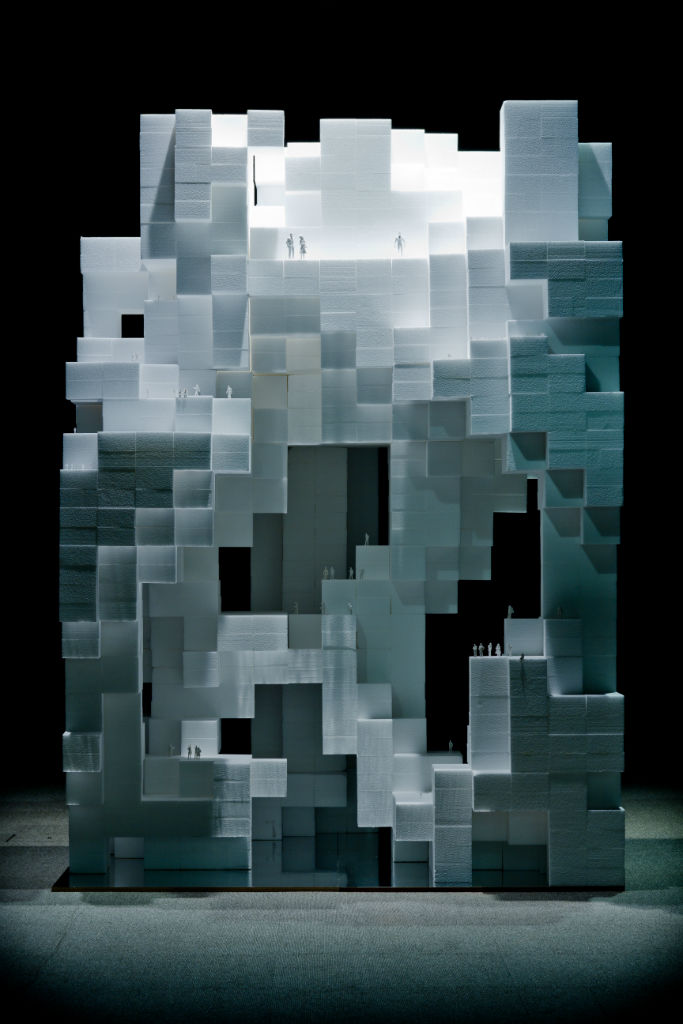
\includegraphics[width=0.5\textwidth]{images/GameOfLife.jpg}
     		\end{center}
		\caption{``Game Of Space'' on exhibit at the Museum of Contemporary Art in Hiroshima.}
	\end{figure}
    	\end{columns}
}

\frame{{Chapter 10}
	\framesubtitle{Cellular Automata, Life, and the Universe}
  Sections:
	\begin{itemize}
	  \item Computation in Nature
    \item Cellular Automata
    \item The Game of Life
    \item The Four Classes
    \item Wolfram's ``A New Kind of Science''
	\end{itemize}
}

\frame{{Computation in Nature}
  \begin{description}
    \item[Q: ]
      In what sense to natural systems \emph{compute}?
    \item[A: ]
      ``At a very general level, one might say that \emph{computation} is what a complex system does with \emph{information} in order to succeed or adapt in its environment.''
  \end{description}
  \begin{block}{A Brief Peek at Chapter 12}
    \begin{itemize}
      \item What plays the role of \emph{information} in the system?
      \item How is it communicated and processed?
      \item How does this information acquire \emph{meaning}?  And to whom?
    \end{itemize}
  \end{block}
}

\frame{{Cellular Automata}
  \begin{block}{Description}
    \begin{itemize}
      \item The CA consists of a regular $n$-dimensional grid of cells.
      \item Each cell can exist in one of a finite number of states.
      \item For each cell, a set of cells called its neighborhood is defined relative to the specified cell.
      \item An initial condition is established by assigning a state for each cell.
      \item A given cell's state is updated according to some fixed rule that determines that cell's new state in terms of its current state and the states of the cells in its neighborhood.
    \end{itemize}
  \end{block}

  Von Neumann was able to show that his cellular automaton was equivalent to a universal Turing machine.
}

\frame{{The Game of Life}
  \begin{block}{Improvement}
    John Conway introduced a 2-state CA capable of universal computation, being able to carry out all the logical combinations of \emph{and}, \emph{or}, and \emph{not}. 
  \end{block}

  \begin{alertblock}{Caveat}
    Despite universality, his CA is not economical in practice.
  \end{alertblock}

  \begin{block}{Goal}
    ``What we really want from cellular automata is to harness their parallelism and ability to form complex patterns in order to achieve computations in a nontraditional way.''
  \end{block}
}

\frame{{The Four Classes}
  Wolfram observed that the behavior of CA fell into four classes.
	\begin{description}
		\item[Class 1: ]
			Quickly settle to the same uniform final pattern independent of initial configuration.
		\item[Class 2: ]
			Produce either a uniform or cyclical patterns that are sensitive to the initial configuration.
		\item[Class 3: ]
			Produce mostly random behavior with some regular structures present.
		\item[Class 4: ]
			A mixture of order and randomness: simple localized structures are produced which interact with each other in complicated ways.
	\end{description}
  Wolfram speculated that all Class 4 CAs are capable of universal computation.
  In the 1990s Matthew Cook proved a special case, Rule 110.
}

\frame{{Wolfram's ``New Kind of Science''}
	Wolfram's proposed principle (in four parts):
	\begin{enumerate}
		\item The proper way to think about processes in nature is that they are \emph{computing}.
		\item Since even very simple rules can support universal computation, the ability to support universal computation is very common in nature.
		\item Universal computation is an upper limit on the complexity of computations in nature.  That is, no natural system or process can produce behavior that is \emph{non-computable}.
		\item The computations done by different processes in nature are almost always equivalent in sophistication.
	\end{enumerate}
}

\frame{{Chapter 11}
	\framesubtitle{Computing with Particles}
  \begin{itemize}
    \item This chapter is illustrated through the example of deciding \emph{majority classification}, where the cellular automaton computes whether its initial configuration contains a majority of \emph{on} or \emph{off} states.
    \item The example represents an interesting class of problems that are, in general, very difficult to solve: those that perform tasks requiring collective decision making among all the cells.
  \end{itemize}
}

\frame{{Manual Approach}
	\begin{columns}[c]
    	\column{.4\textwidth}
  Mitchell describes a manual attempt that uses the \emph{local majority} to determine the state of any given cell.  While this sounds like it might be a reasonable approach, it fails to resolve boundaries.
    	\column{.6\textwidth}
  \begin{center}
    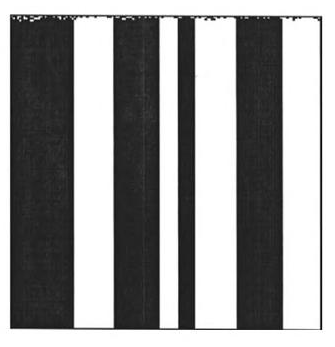
\includegraphics[scale=0.5]{images/ManualTry.png}
  \end{center}
  \end{columns}
}

\frame{{Genetic Approach}
	\begin{itemize}
    \item Begin with a population of randomly generated CA rules.
    \item Each rule is tested against many different initial configurations.
    \item Fitness is determined on the number of correct final evaluations.
    \item Successive generations are based on the rules with highest fitness.
    \item The author does not indicate how successive generations are evolved.
	\end{itemize}
}

\frame{{Results}
  The following figure shows the results of successful rule sets in determining majority black and majority white initial lattice.
  \begin{center}
    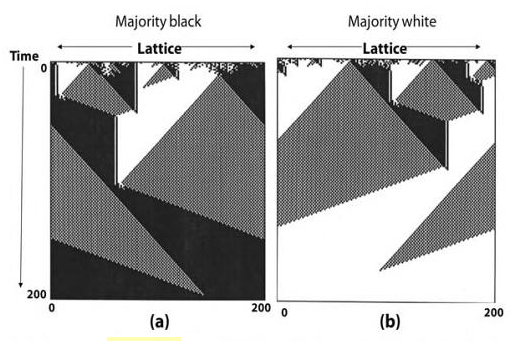
\includegraphics[scale=0.5]{images/BlackWhiteLattice.png}
  \end{center}

}

\frame{{Interpretation}
	\begin{columns}[c]
  \column{.6\textwidth}
  Looking closely at the space-time diagram we discover some patterns emerge
  \begin{itemize}
    \item Homogeneous regions converge quickly.
    \item Whenever a black region on the left meets a white region on the right, a vertical boundary results.
    \item The opposite results in a checkerboard triangle.
  \end{itemize}
  Much can be understood by observing the edges marked \emph{Side A} and \emph{Side B}.  Since they grow at the same rate, the one with the shorter distance to travel exerts less influence.
  \column{.4\textwidth}
  \begin{center}
    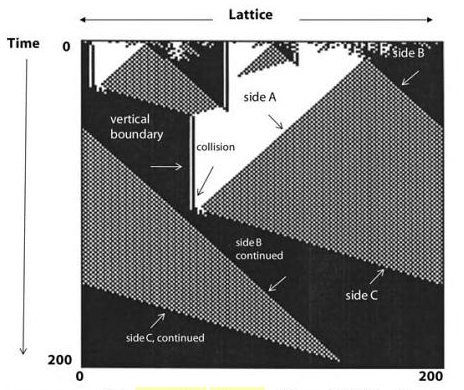
\includegraphics[scale=0.3]{images/CloseUp.png}
  \end{center}
  \end{columns}
}

\frame{{Signals}
  ``If we try to understand these patterns as carrying out a computation, then the vertical boundary and the checkerboard region can be thought of as \emph{signals}.  These signals are created and propagated by local interactions among cells.  The signals are what allow the cellular automaton as a whole to determine the relative sizes of the larger-scale adjacent black and white regions, cut off the smaller ones, and allow the larger ones to grow in size.''

  \hfill-- Mitchell
}

\frame{{Consequences}
	\begin{center}
    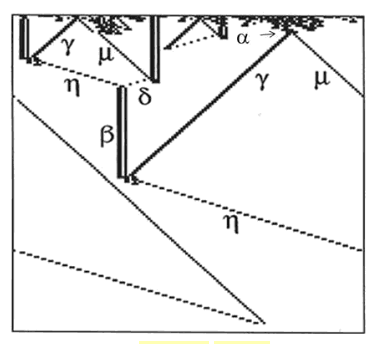
\includegraphics[scale=0.35]{images/Particles.png}
  \end{center}
  Interactions of the boundaries (or edges) between regions can be explained within this particle metaphor.
  \begin{itemize}
    \item The CA produces six types of particles: $\gamma$, $\mu$, $\eta$, $\delta$, $\beta$, and $\alpha$.
    \item $\beta+\gamma, \mu+\beta,$ and $\eta+\delta$ create a new particle.
    \item $\eta+\mu$ and $\gamma+\delta$ result in annihilation.
  \end{itemize}
}

\frame{{Questions?}
	\begin{center}
		
\includegraphics[width=.7\textwidth]{images/fin.png}
	\end{center}
}

\end{document}
